\quad Al igual que en el an\'alisis previo, realizamos mediciones de los estimadores variando el par\'ametro de entrada sobre las mismas poblaciones mencionadas.\\

\quad El par\'ametro que se var\'ia en todos los estimadores representa la cantidad de \textit{buckets}, aunque en el estimador de pasos distribuidos lo llaman \textit{steps}. \\

\quad Se realizaron las comparaciones con un m\'etodo exacto calculado sobre la colecci\'on de datos testeados.

\subsubsection{Distribuci\'on uniforme}

\begin{itemize}
\item \textbf{Operaci\'on por igualdad} \\

\begin{figure}[H]
	  \begin{center}
	    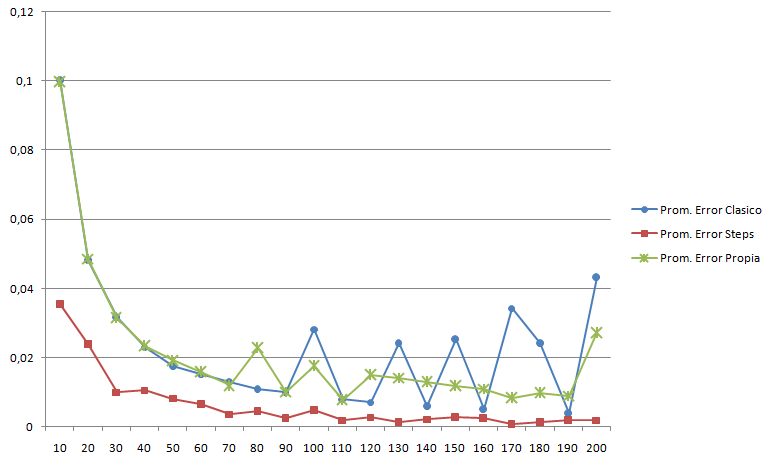
\includegraphics[scale=.80]{imagenes/parametroVariableC0Eq.png}
	    \caption{Error promedio de la Columna C0 de la tabla brindada por la materia} 
	    \label{fig:C0_variando_parametro}
	  \end{center}
\end{figure}

\quad En la figura, se ve claramente como aumentando la cantidad de buckets el error disminuye. Esto se debe a que, al aumentar la cantidad de buckets, se aumenta la granuralidad sobre el rango de valores. Se puede apreciar como para el histograma cl\'asico y el estimador de grupo afecta todav\'ia mucho m\'as que con el de pasos distribuidos. En \'este \'ultimo, al principio mejora bastante (hasta los 70 buckets) pero se estabiliza en un cierto valor y deja de mejorar. En cambio. con los otros dos va mejorando pero se puede ver como se vuelve inestable para ciertos valores del par\'ametro. Creemos que se debe a ciertos casos bordes con respecto a la cantidad de elementos y los valores presentes de un rango y la cantidad de buckets. \\

\item \textbf{Operaci\'on por mayor} \\

\quad Ahora los estimadores los mediremos por su selectividad en un rango buscando ciertos valores en las distribuciones fijos y variando el par\'ametro. \\

\begin{figure}[H]
	  \begin{center}
	    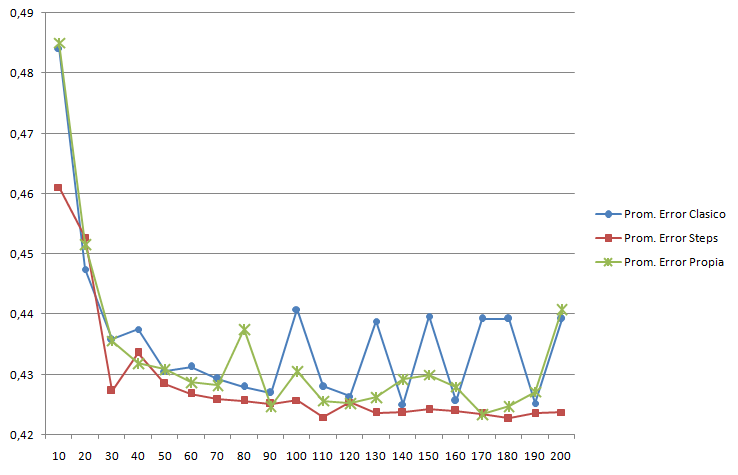
\includegraphics[scale=.80]{imagenes/parametroVariableC0Greater.png}
	    \caption{Error promedio de la Columna C0 de la tabla brindada por la materia} 
	    \label{fig:C0_variando_parametro_greater}
	  \end{center}
\end{figure}

\quad Podemos apreciar la similitudes entre este gr\'afico y el de la Figura	 \ref{fig:C0_variando_parametro}. Pero los valores de error son mucho mayores. \'Esto se debe a que se acumula error, que si bien puede pasar que entre errores se cancelen, creemos que en este caso se acumulan. A pesar de esto, consideramos correcto que mantengan la \textit{forma} ambos gr\'aficos.

\quad Al igual que en el gr\'afico anterior, notamos como el histograma cl\'asico y el estimador propio son inestables. Adem\'as, vuelve a pasar lo mismo con el de pasos distribuidos, mejora hasta cierto punto donde luego de determinado valor del par\'ametro tiende a un valor fijo.

\quad De estos gr\'aficos podemos concluir que para las distribuciones uniformes, el que \textit{mejor} se comporta es el estimador de pasos distribuidos debido a su estabilidad y menor valor de error.

\end{itemize}

\subsubsection{Distribuci\'on normal}

\begin{itemize}
\item \textbf{Operaci\'on por igualdad} \\

\quad Usando la misma metodolog\'ia de tests, analisaremos para colecci\'on de datos con distribuci\'on normal. \\

\begin{figure}[H]
	  \begin{center}
	    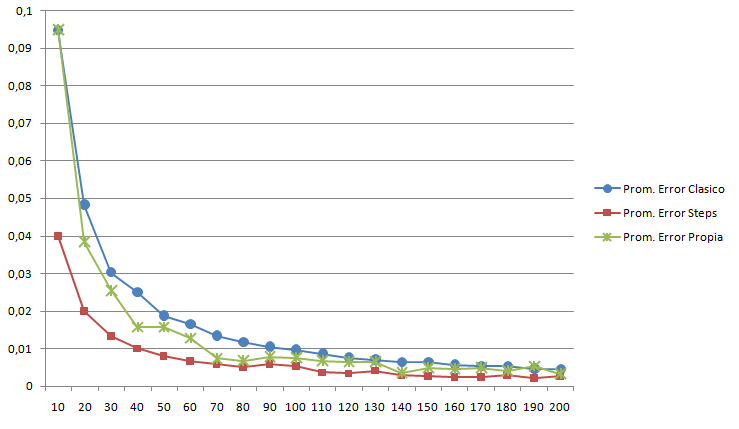
\includegraphics[scale=.80]{imagenes/parametroVariableC2Eq.png}
	    \caption{Error promedio de la Columna C2 de la tabla brindada por la materia} 
	    \label{fig:C2_variando_paremetro}
	  \end{center}
\end{figure}

\quad Nuevamente, todos mejoran a medida de que se aumenta la cantidad de buckets. Pero, en este caso, los tres son estables y, llamativamente, convergen hacia un mismo valor de error. Es decir, que a partir de cierto punto, no hay diferencia apreciable en cuanto al error entre los tres estimadores. Particularmente, cuando la cantidad de buckets es igual a 200, por el gr\'afico se ve que la diferencia entre los estimadores es menor a 0,0025 aproximadamente.\\

\item \textbf{Operaci\'on por mayor} \\

\begin{figure}[H]
	  \begin{center}
	    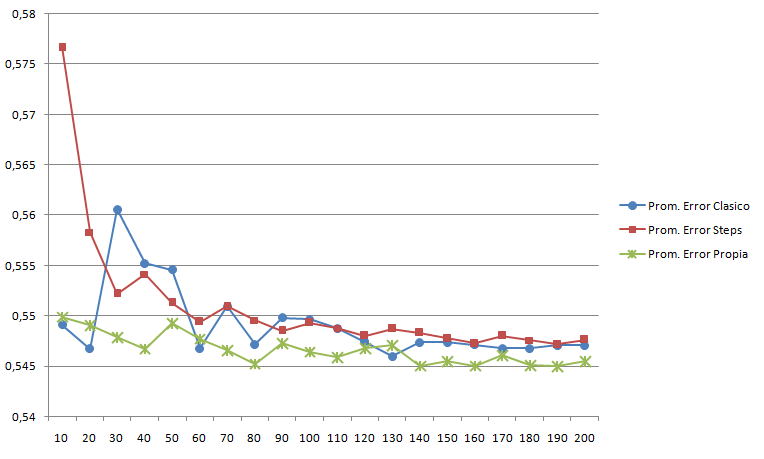
\includegraphics[scale=.80]{imagenes/parametroVariableC2Greater.png}
	    \caption{Error promedio de la Columna C2 de la tabla brindada por la materia} 
	    \label{fig:C2_variando_paremetro_greater}
	  \end{center}
\end{figure}

\quad En esta figura, vemos como el que empieza con mayor error es el de pasos distribuidos y al igual que los otros dos va disminuyendo el error a medida que se incrementa la cantidad de buckets. Con respecto al de histograma cl\'asico, empieza inestable y luego se estabiliza, ocurr\'ia lo contrario en los gr\'aficos \ref{fig:C0_variando_parametro} y \ref{fig:C0_variando_parametro_greater}. En cuanto al estimador propio, vemos que no es tan significativa la mejora compar\'andola con los otros dos pero es el que menor error genera. \\

\quad Se ve que, en este caso, los resultados dieron muy diferentes a todos los anteriores gr\'aficos. Mostrando como, los estimadores dependen del tipo de distribuci\'on y, adem\'as, del tipo de operaci\'on que se realice \\

\end{itemize}